\documentclass{article}
\usepackage{graphicx} % Required for inserting images
\usepackage{float}
\usepackage{amsmath}
\usepackage{subcaption}
\usepackage{xcolor}
\usepackage{amssymb}

\title{ELEN 3201 Circuit Analysis Experiment 4}
\author{Songhang Li}
\date{November 2025}

\begin{document}

\maketitle


\section{Part 1}

\subsection{(a)}

Given, \[\begin{gathered}
R_1=R_2=R_3=R_4=R_5=R_6=R_7=R_8=1 \mathrm{M} \Omega \\
C_1=C_2=1 \mu \mathrm{~F}
\end{gathered}\]
 we have the following
 \[
w_0=\sqrt{\frac{K_1}{\tau_1 \tau_2}}=\sqrt{\frac{R_5}{R_6} \cdot \frac{1}{R_1 C_1 R_2 C_2}}=1
\]

\[\begin{aligned}
& \alpha=\zeta \omega_0=\frac{1}{2} \cdot 1=\frac{1}{2} \\
& \omega_d=\sqrt{\omega_0^2-\alpha^2}=\frac{\sqrt{3}}{2}
\end{aligned}\]

\[\begin{aligned}
& w_0 / Q=K_3 / \tau_1 \\
& Q=\frac{w_0 \cdot \tau_1}{K_3}=\frac{1}{2} \Rightarrow \\
& \xi=0.5 <1
\end{aligned}\]


\[2 \zeta \omega_0=1 \Rightarrow 2 \zeta(1)=1 \Rightarrow \zeta=0.5 \text{~so it is underdamped}\]


Initial conditions
\[\begin{aligned}
& V_{C_2}(0^-)=V_{C_2}\left(0^{+}\right)=0 \\
& \frac{d V_{C_1}(0)}{d t}=0
\end{aligned}\]


\[x(t)^{\prime}=\frac{1}{2} e^{-t / 2}\left[(\sqrt{3} \mathrm{~B_2}-\mathrm{B}_1) \cos \left(\frac{\sqrt{3} t}{2}\right)-(\sqrt{3} \mathrm{~B}_1+\mathrm{B}_2) \sin \left(\frac{\sqrt{3} t}{2}\right)\right]\]


\[\left(\sqrt{3} B_2-B_1\right)=0 \quad \sqrt{3} \quad B_1=-1 \quad \Rightarrow B_2=-\frac{1}{\sqrt{3}}\]


\[\begin{aligned}
&\text { Underdamped }\left(\zeta<1 \text { or } \alpha<\omega_0\right) \text { : }\\
&y_n(t)=e^{-\alpha t}\left(B_1 \cos \omega_d t+B_2 \sin \omega_d t\right)\\
&y = y_n+ y_f = e^{-\alpha t}\left(B_1 \cos \omega_d t+B_2 \sin \omega_d t\right) + 1
\end{aligned}\]

\[\begin{gathered}
s_1, s_2=-\alpha \pm\left(\alpha^2-\omega_0^2\right)^{1 / 2} \\
\omega_d=\left(\omega_0^2-\alpha^2\right)^{1 / 2}
\end{gathered}\]




Therefore, 
\[x(t)=1-e^{-0.5 t}\left[\cos \left(\frac{\sqrt{3}}{2} t\right)+\frac{1}{\sqrt{3}} \sin \left(\frac{\sqrt{3}}{2} t\right)\right]\]

\begin{figure}
    \centering
    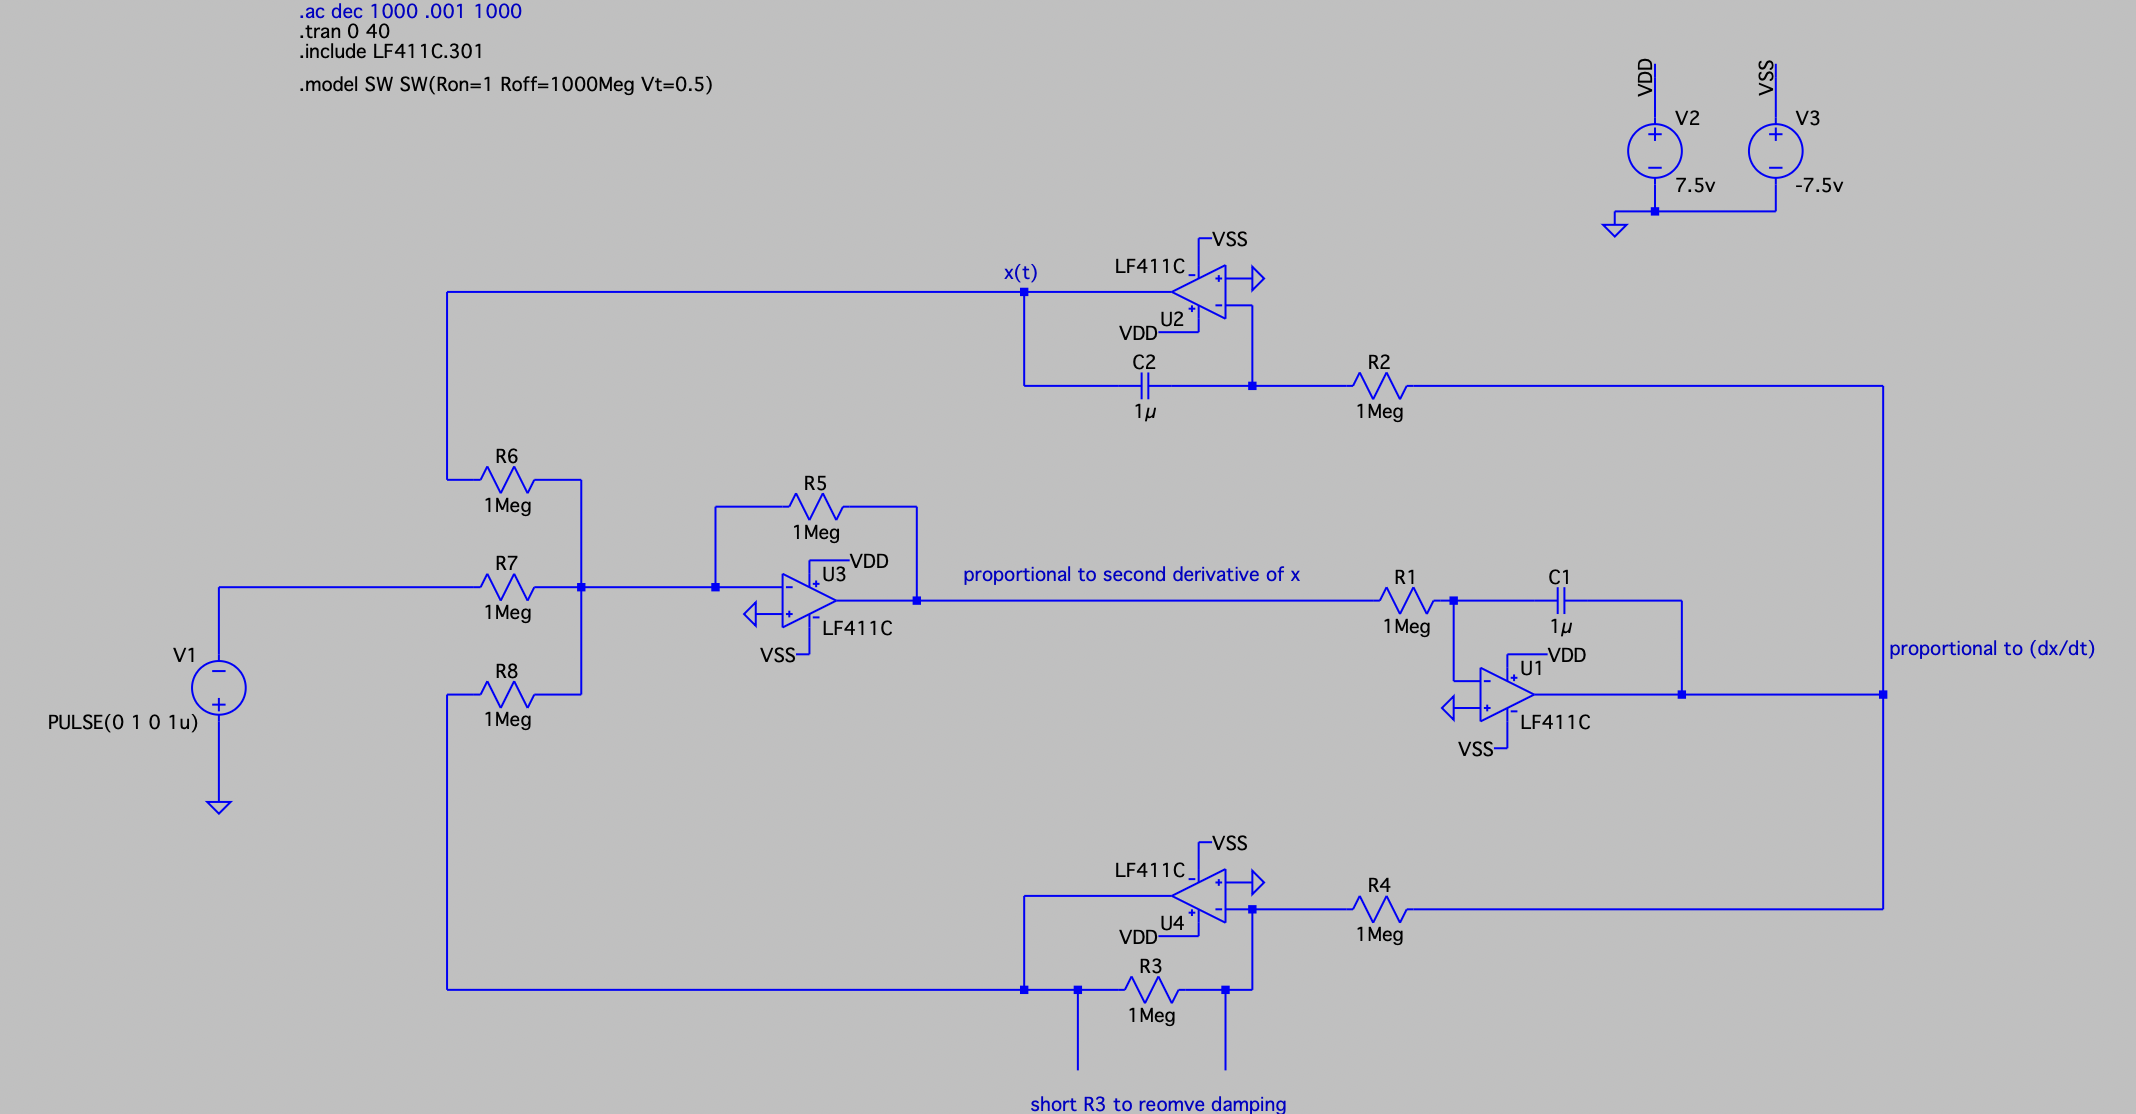
\includegraphics[width=0.75\linewidth]{part1Schematic.png}
    \caption{Part 1 Schematic}
    \label{fig:placeholder}
\end{figure}

\begin{figure}[H]
    \centering
    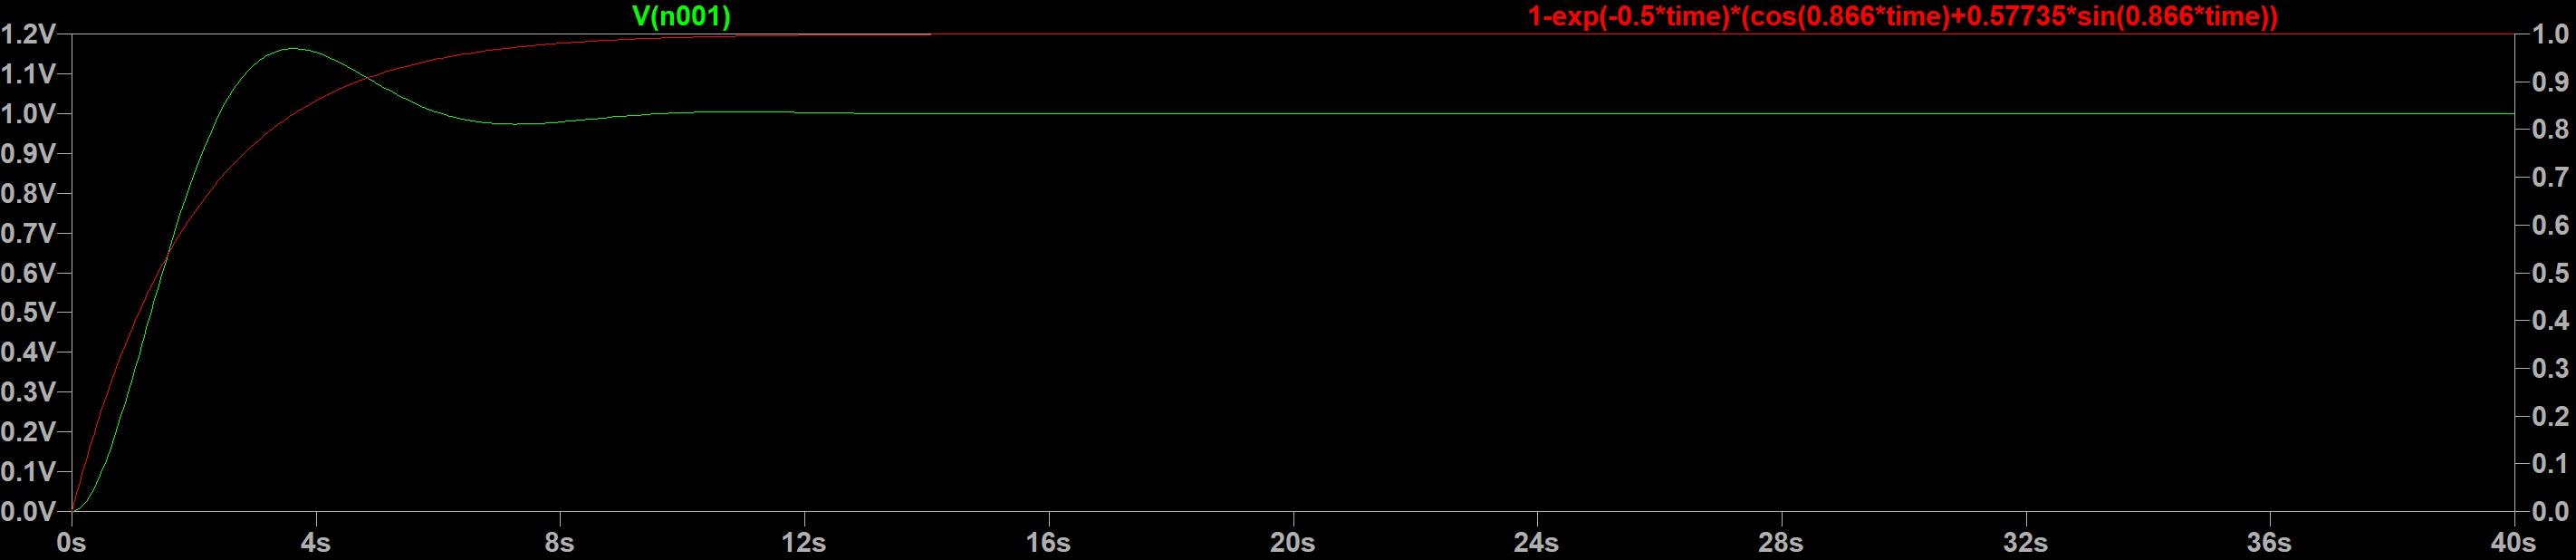
\includegraphics[width=1\linewidth]{part1aSimulation.png}
    \caption{part 1a $\color{green}\text{simulation(green)}$ \& $\color{red} \text{ideal(red)}$}
    \label{fig:placeholder}
\end{figure}

\begin{figure}[H]
    \centering
    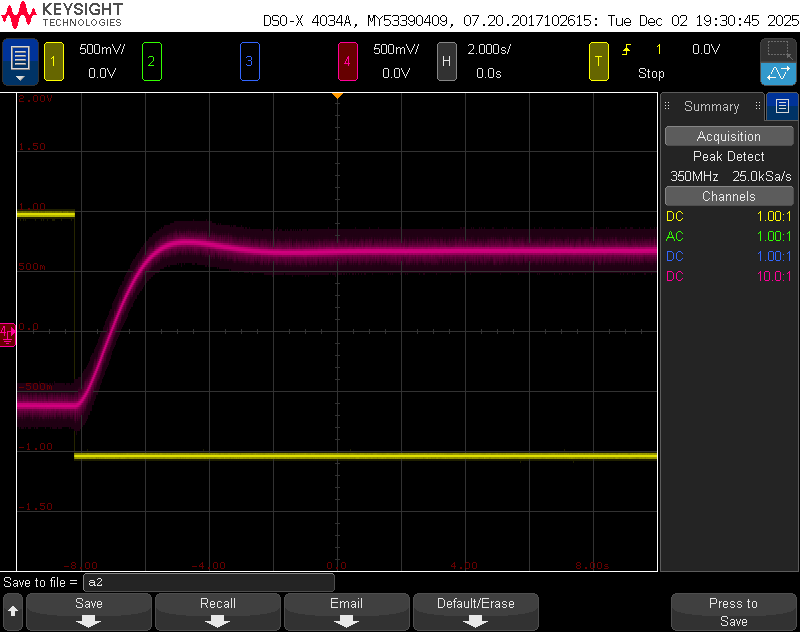
\includegraphics[width=0.5\linewidth]{part1aMeasurement.png}
    \caption{Part 1 a measurement}
    \label{fig:placeholder}
\end{figure}



\subsection{(b) shorting $R_3$}

\begin{figure}[H]
    \centering
    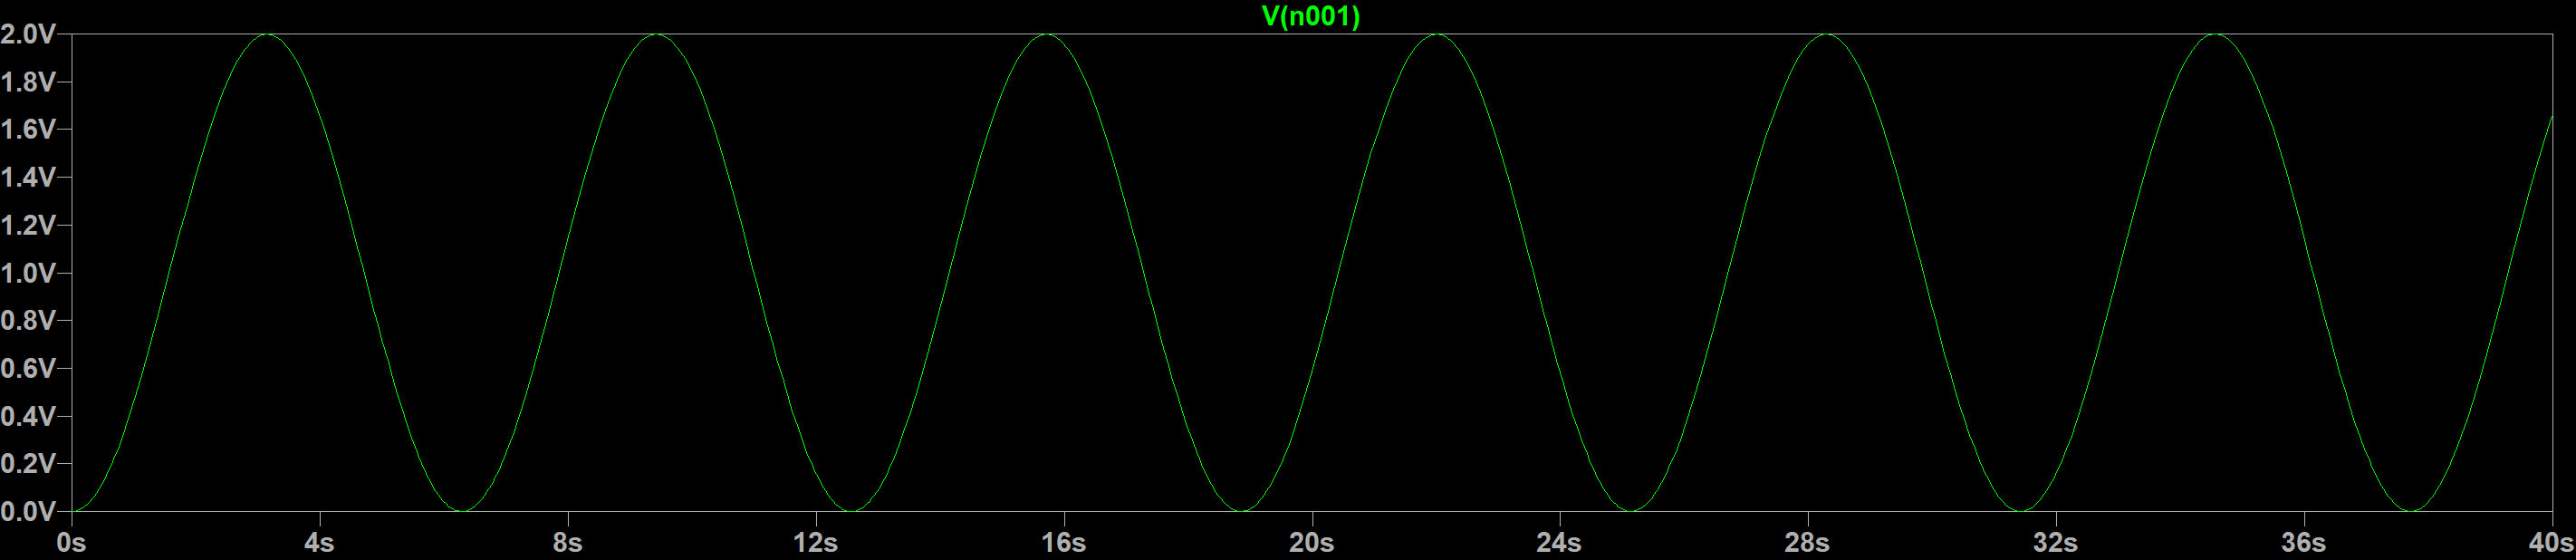
\includegraphics[width=1\linewidth]{part1bSimulation.png}
    \caption{part1 b simulation: shorting R3}
    \label{fig:placeholder}
\end{figure}


\textit{What does shorting R3 do to the damping factor?}

The damping factor becomes zero, thus the decaying component of the solution disappears and result oscillates forever(theoratically).


\begin{figure}[H]
    \centering
    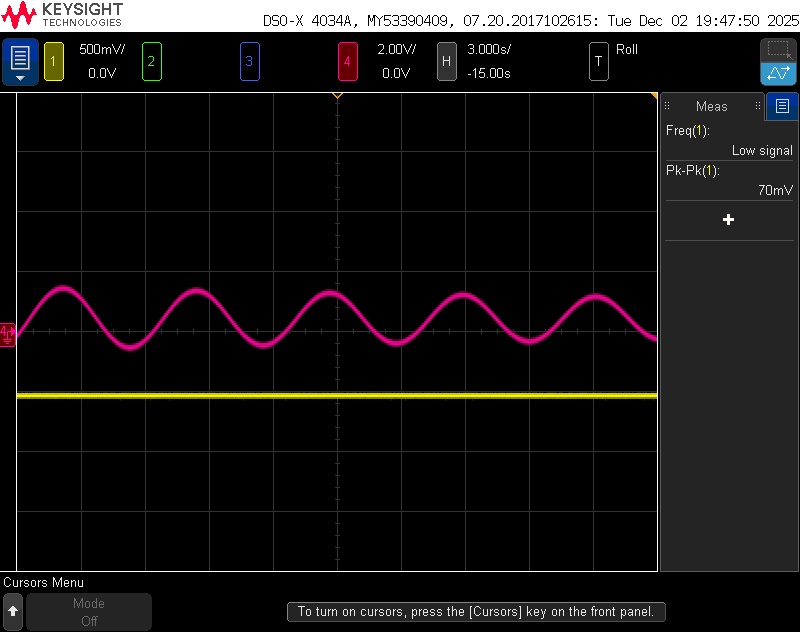
\includegraphics[width=0.5\linewidth]{partbMeasurement.png}
    \caption{part b measurement}
    \label{fig:placeholder}
\end{figure}

\subsection{(c) $R_3$ making critically damped}

We need \(\xi=1\)

\[
\zeta=1 \Rightarrow Q=\frac{1}{2 \zeta}=\frac{1}{2}=\frac{1}{K_3} \Rightarrow \quad K_3=2 \Rightarrow \color{red}R_3=2 \mathrm{M}\Omega .
\]


\begin{figure}[H]
    \centering
    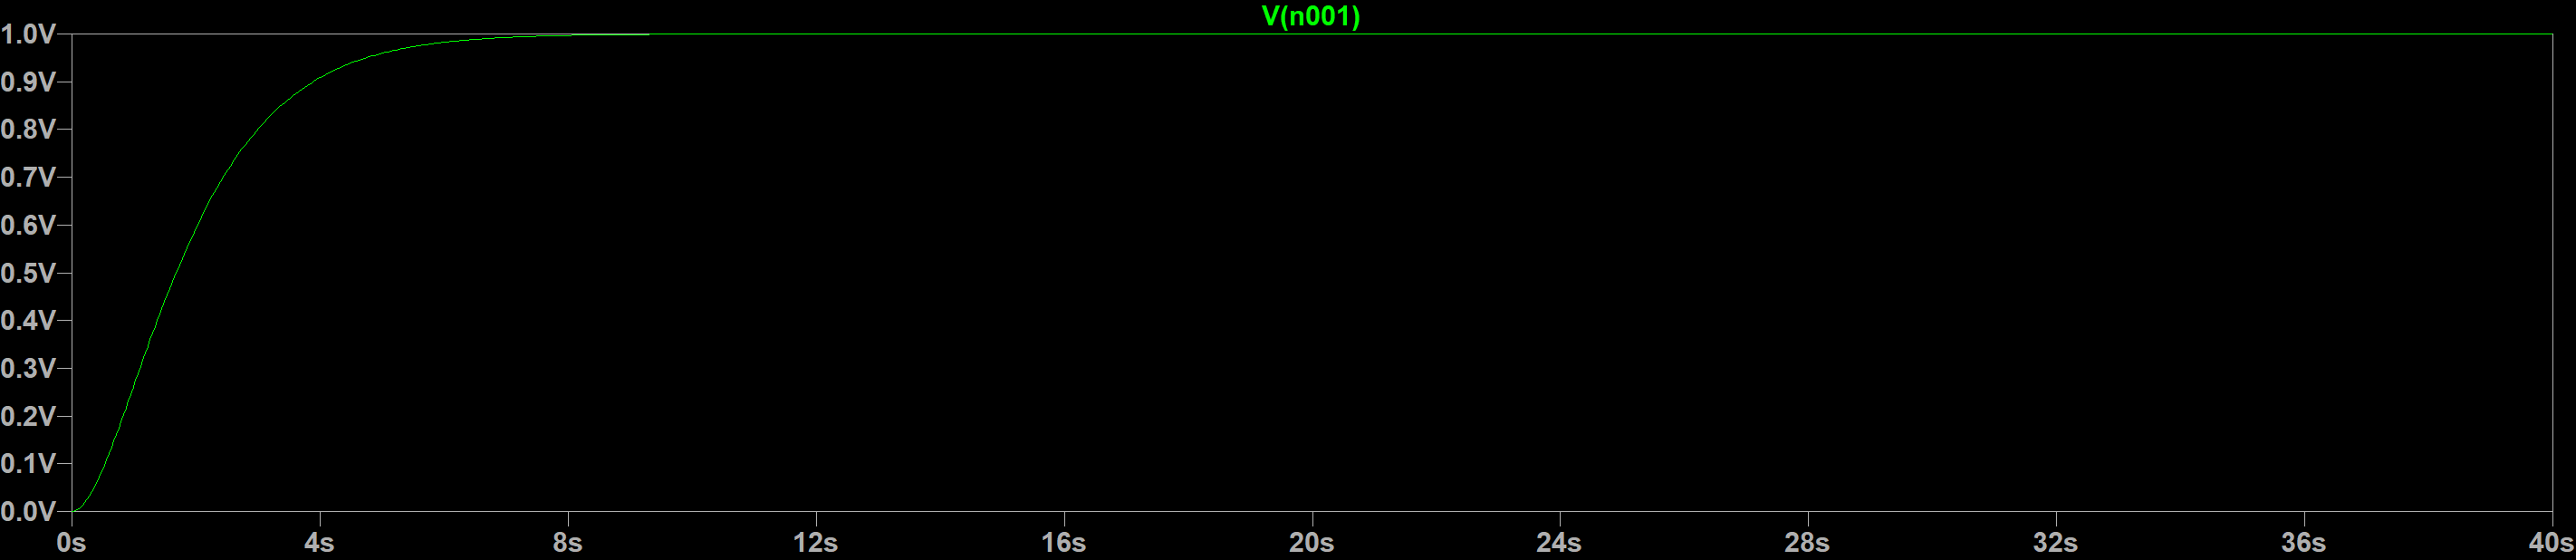
\includegraphics[width=1\linewidth]{part1cSimulation.png}
    \caption{part 1c Simulation Critically damped (\(R_3 = 2 \mathrm{M}\Omega\))}
    \label{fig:placeholder}
\end{figure}

\begin{figure}[H]
    \centering
    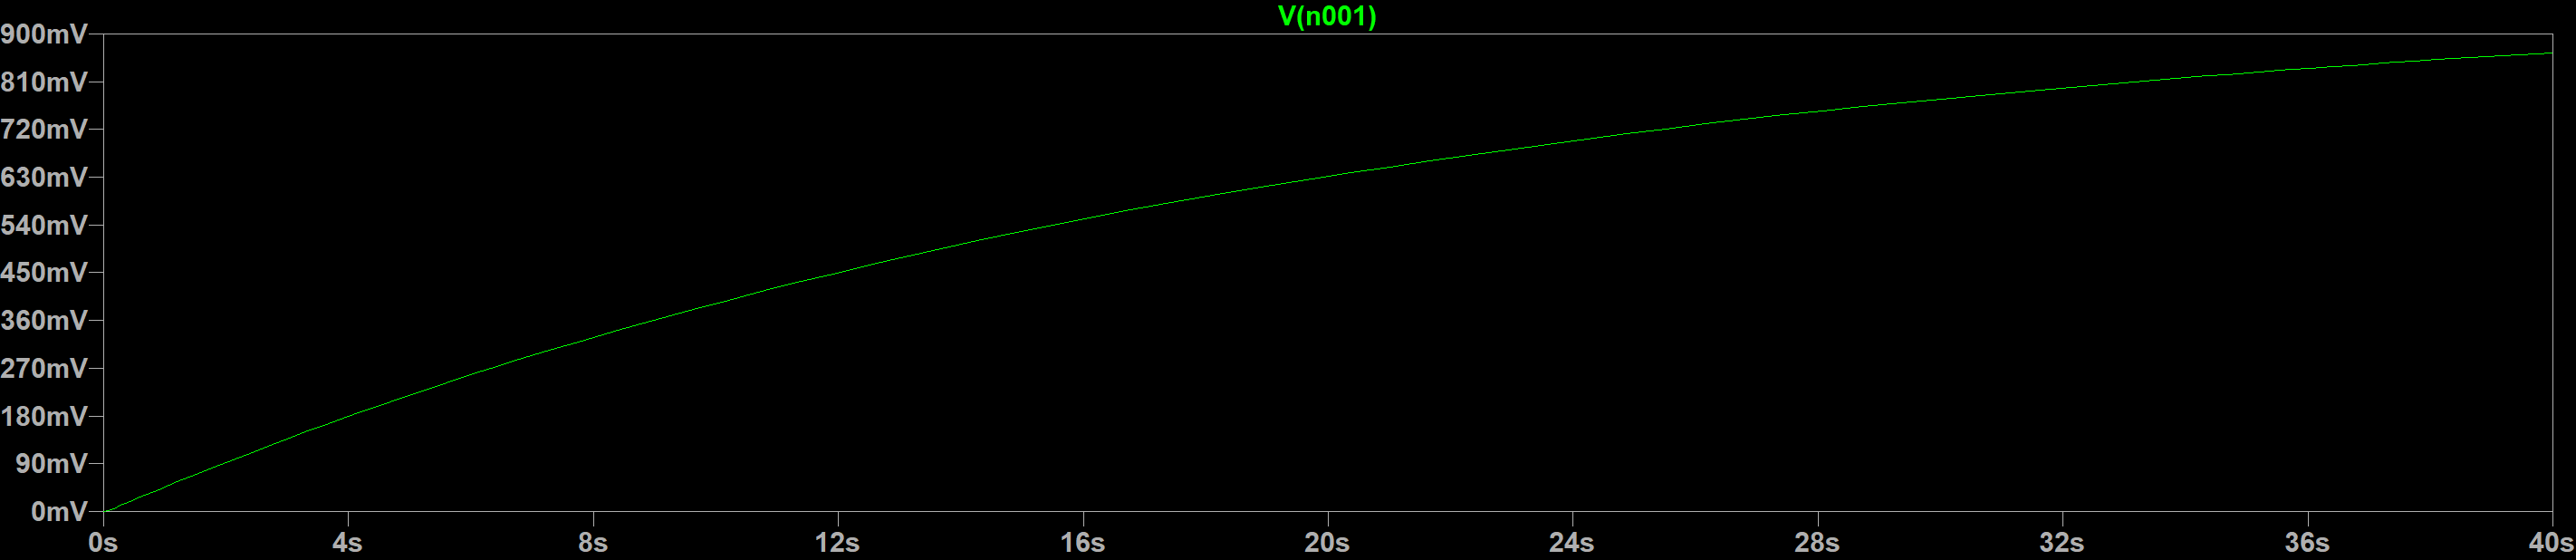
\includegraphics[width=1\linewidth]{part1cSimulation10x.png}
    \caption{part1c Simulation 10x: Overdamped (\(R_3 = 20 \mathrm{M}\Omega\))}
    \label{fig:placeholder}
\end{figure}

\begin{figure}[H]
    \centering
    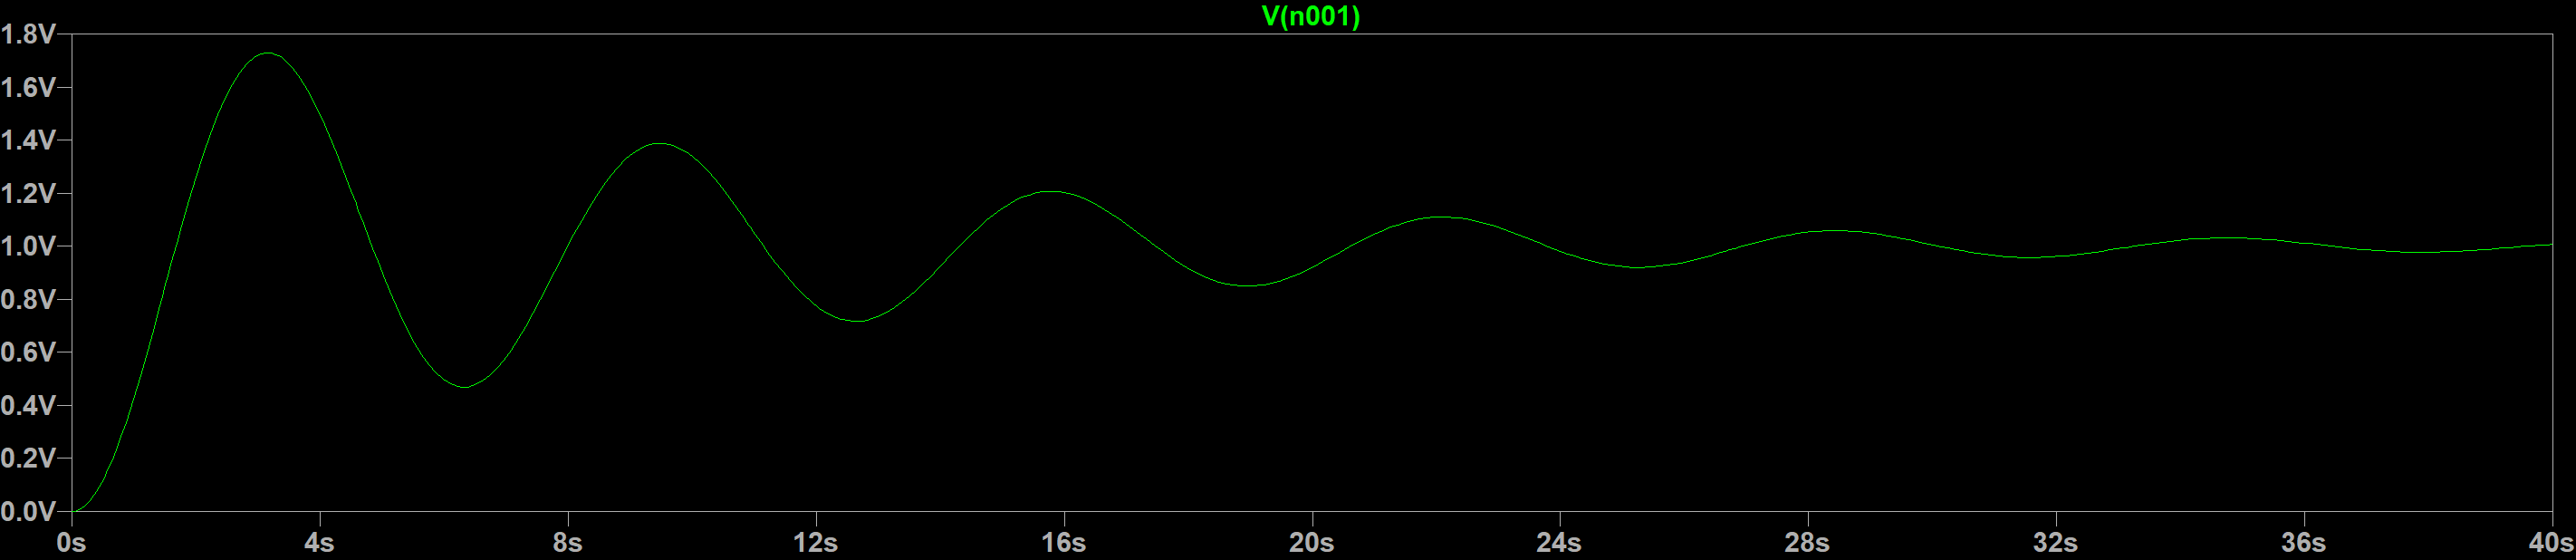
\includegraphics[width=1\linewidth]{part1cSimulation0.1x.png}
    \caption{part 1c Simulation 0.1x: Underdamped (\(R_3 = 0.2 \mathrm{M}\Omega\))}
    \label{fig:placeholder}
\end{figure}

\begin{figure}[H]
    \centering
    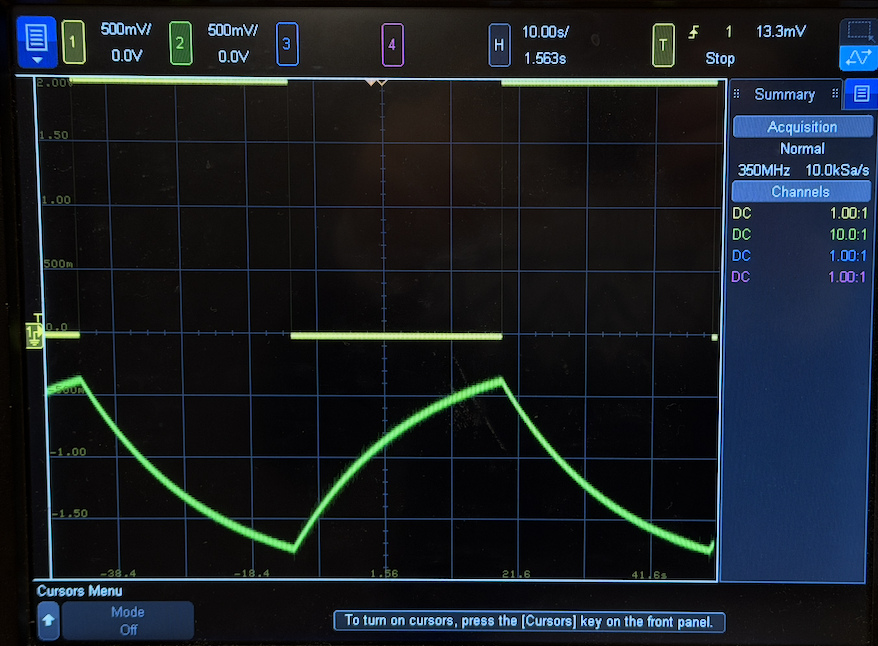
\includegraphics[width=0.5\linewidth]{part1cMsrmt_underdamped.png}
    \caption{part 1 c overdamped measurement}
    \label{fig:placeholder}
\end{figure}


\begin{figure}[H]
    \centering
    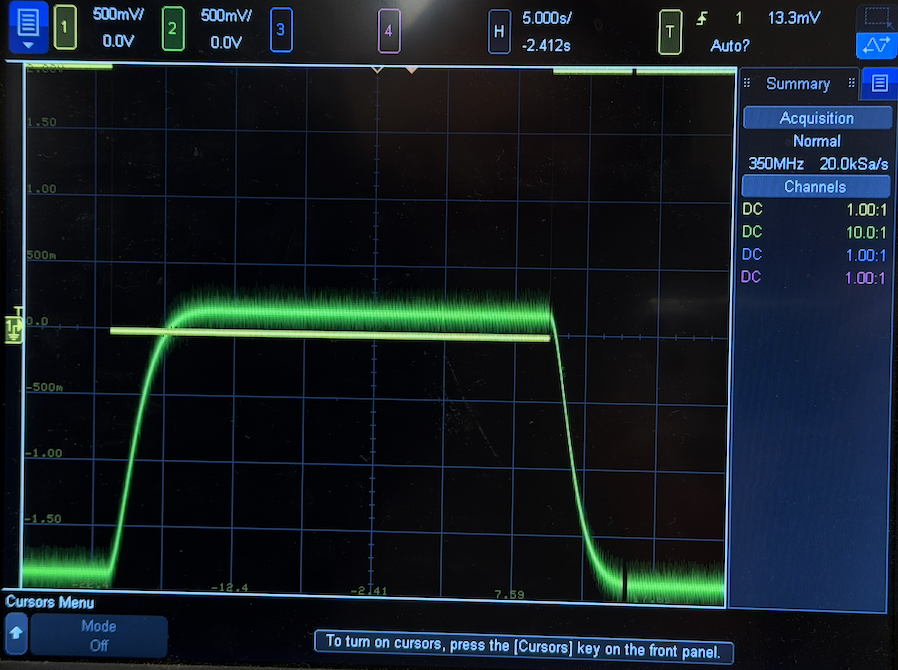
\includegraphics[width=0.5\linewidth]{part1cMrmt_criticallydamped.png}
    \caption{part 1 c critically damped}
    \label{fig:placeholder}
\end{figure}


\begin{figure}[H]
    \centering
    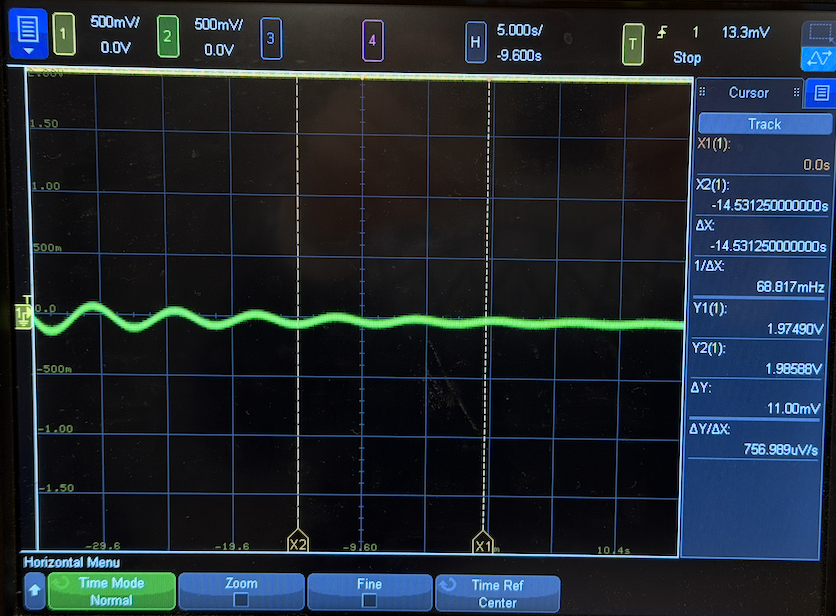
\includegraphics[width=0.5\linewidth]{part1cMrsm_Underdamped.png}
    \caption{part 1 c underdamped}
    \label{fig:placeholder}
\end{figure}



\begin{figure}[H]
    \centering
    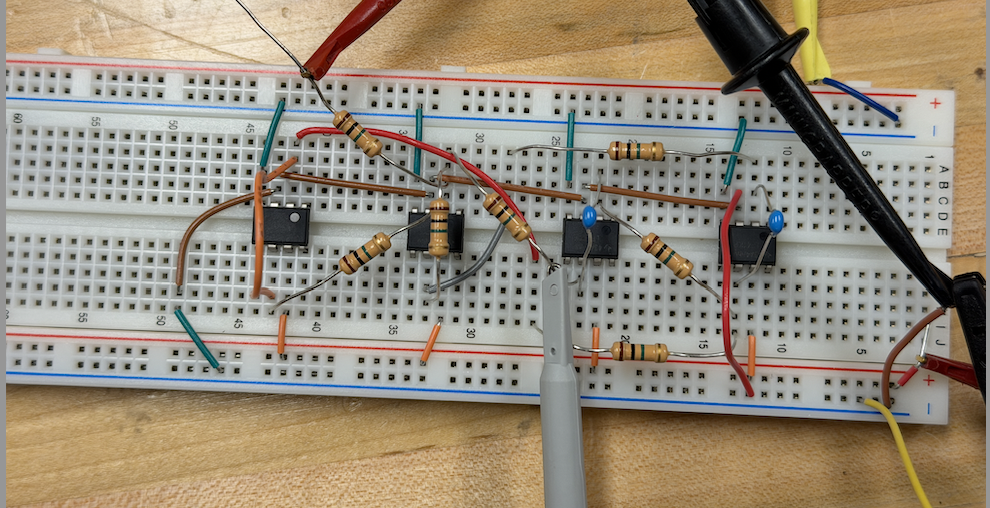
\includegraphics[width=0.5\linewidth]{part1cCircuit.png}
    \caption{1c circuit}
    \label{fig:placeholder}
\end{figure}


\subsection{(d) $\omega_0 = 100 $}

Again, \(\color{red}Q=\frac{1}{2}\) is needed for the system to be critically damped because \(Q=\frac{1}{2 \zeta}=w_0 \cdot \frac{\tau_1}{K_3}=\frac{1}{2}\). As \(\omega_0 \times 100\), we need to make \(\color{red}K_3 =200 \) so that Q remains \(\frac{1}{2}\), i.e. \(\color{red}100 \color{black} \cdot \frac{\tau_1}{\color{red}200}=\frac{1}{2}\).

Furthermore, to minimize the adjustment of the circuit, we chose the capacitor \(C_2\) to be \(10^{-4}\) smaller than the original to accommodate the change of \(K_3\) while keeping \(C_1\) the same( so \( \tau_1\) does not need to change).

\[
w_0=\sqrt{\frac{R_1}{\tau_1 \tau_2}}=\sqrt{\frac{R_5}{R_6} \cdot \frac{1}{R_1 C_1 R_2 C_2}} \Rightarrow \text{ adjust }C_1, C_2 
\]

\[
\Rightarrow C_1 \text{ not changed}, \quad  C_2 \times 10^{-4} (\color{red} C_2=0.1 \mathrm{~nF}\color{black}) \text{ to set } \omega_0=100.
\]
Next, picking the resistors,
\[
K_3=\frac{R_3 R_5}{R_4 R_8}=200 \Rightarrow \frac{R_3}{R_4}=200 \text{ (and } 2 k \Omega \leqslant R_3=200 R_4 \leqslant 10 \mathrm{M} \Omega) .
\]

We picked \(\color{red}R_4 = 2 k \Omega\) and \( \color{red}R_3 = 400k\Omega, 40k\Omega, 4\mathrm{M} \Omega\)  (critically damped, underdamped, overdamped, respectively)

The rest of the components remain the same.

\begin{figure}[H]
    \centering
    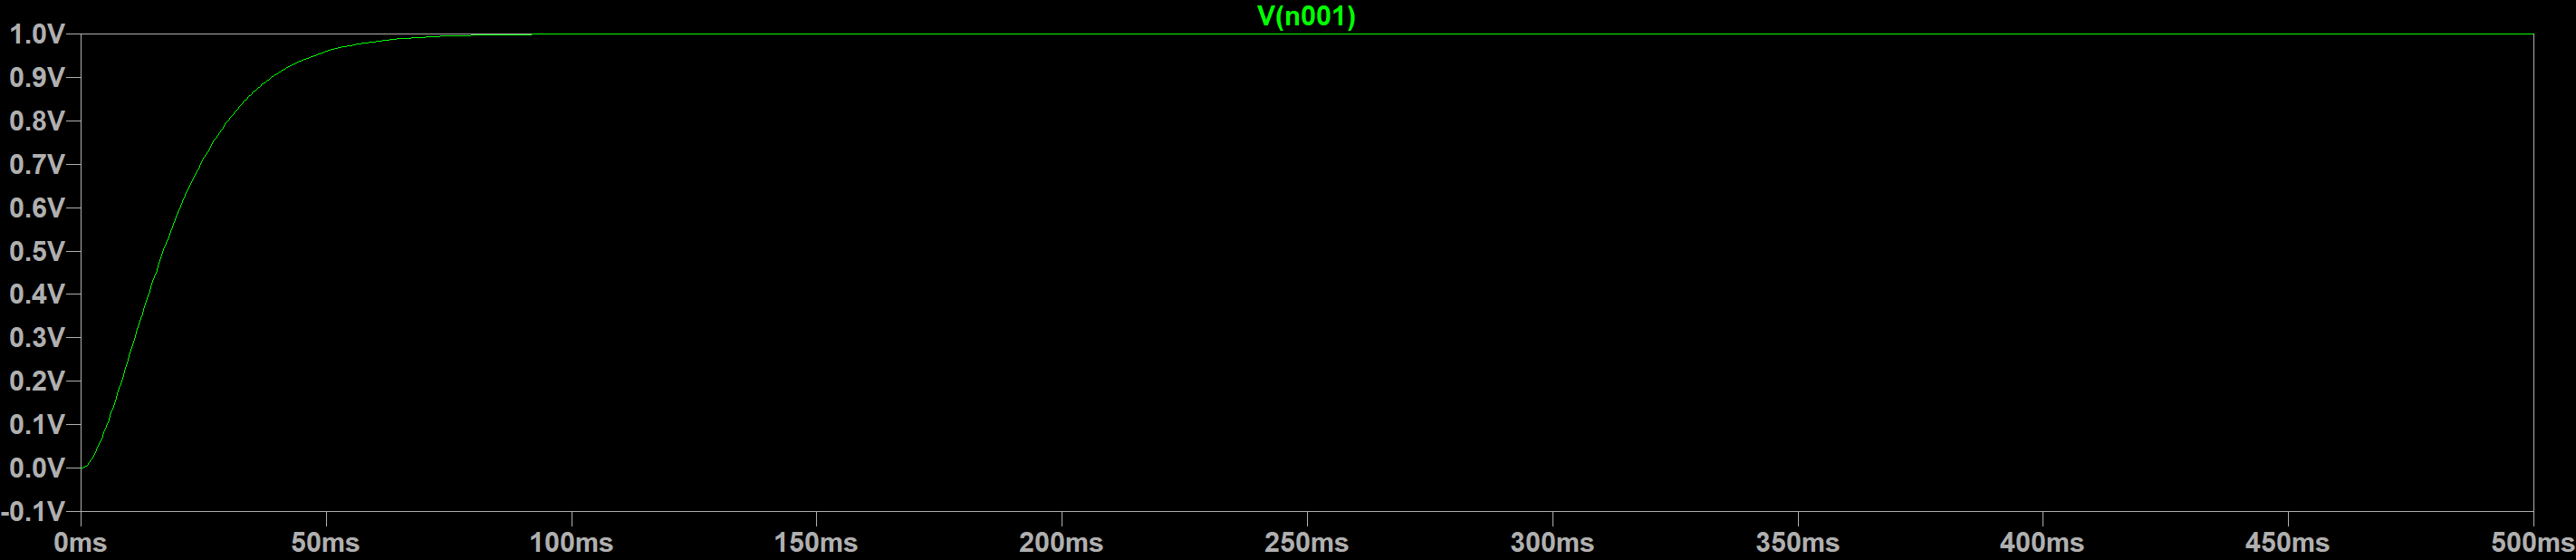
\includegraphics[width=1\linewidth]{partd_critDamped.png}
    \caption{R3 = 400k critically damped}
    \label{fig:placeholder}
\end{figure}


\begin{figure}[H]
    \centering
    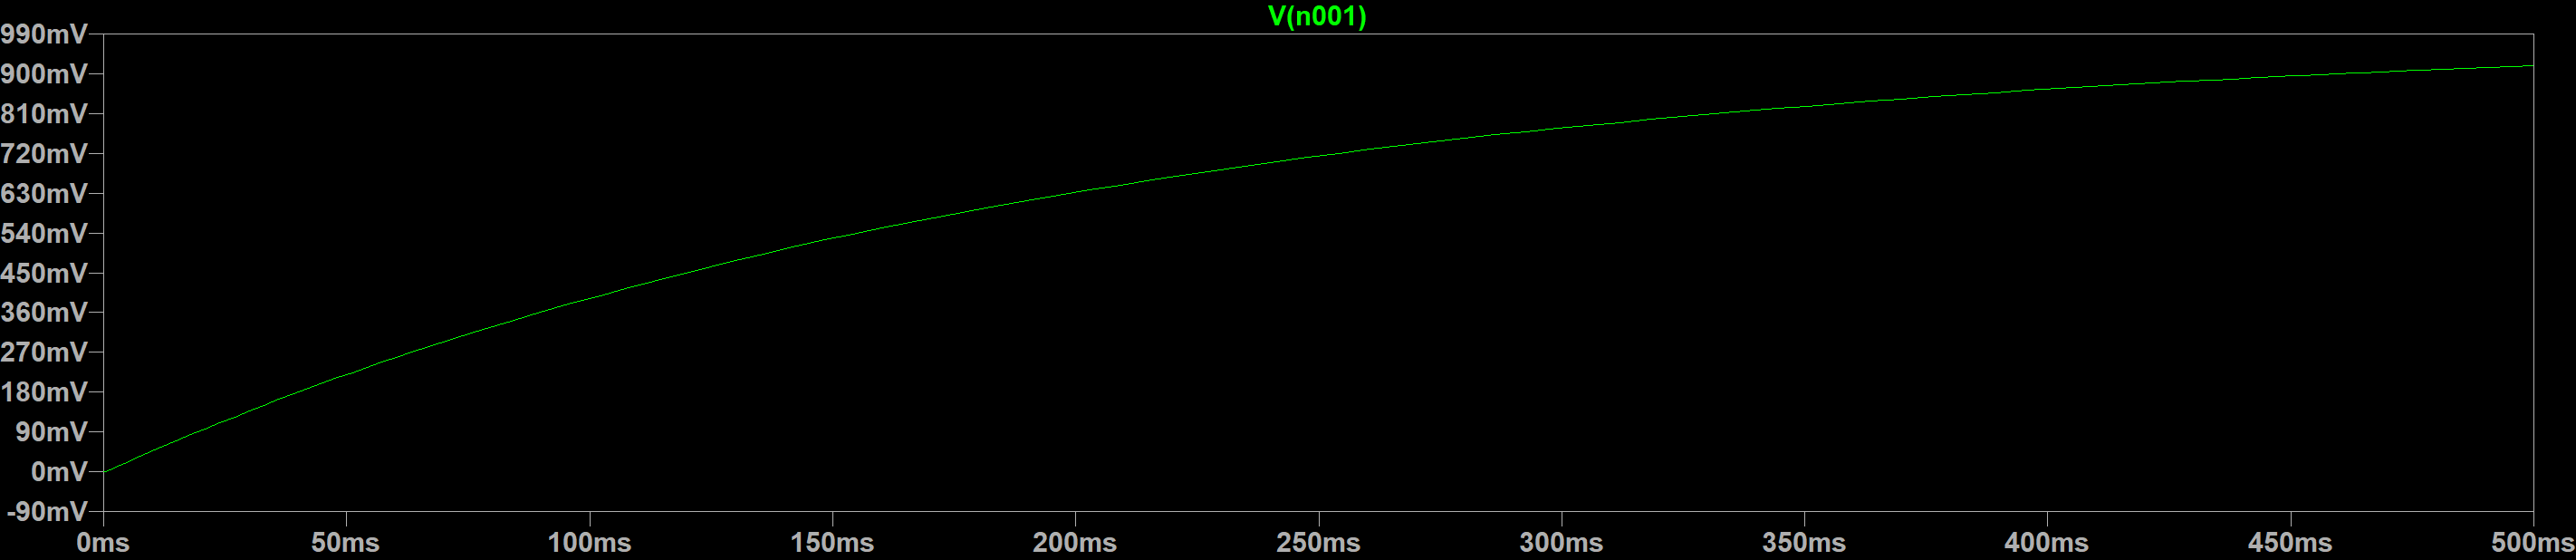
\includegraphics[width=1\linewidth]{partd_ovrDamped.png}
    \caption{over damped R3=4M\(\Omega\)}
    \label{fig:placeholder}
\end{figure}

\begin{figure}[H]
    \centering
    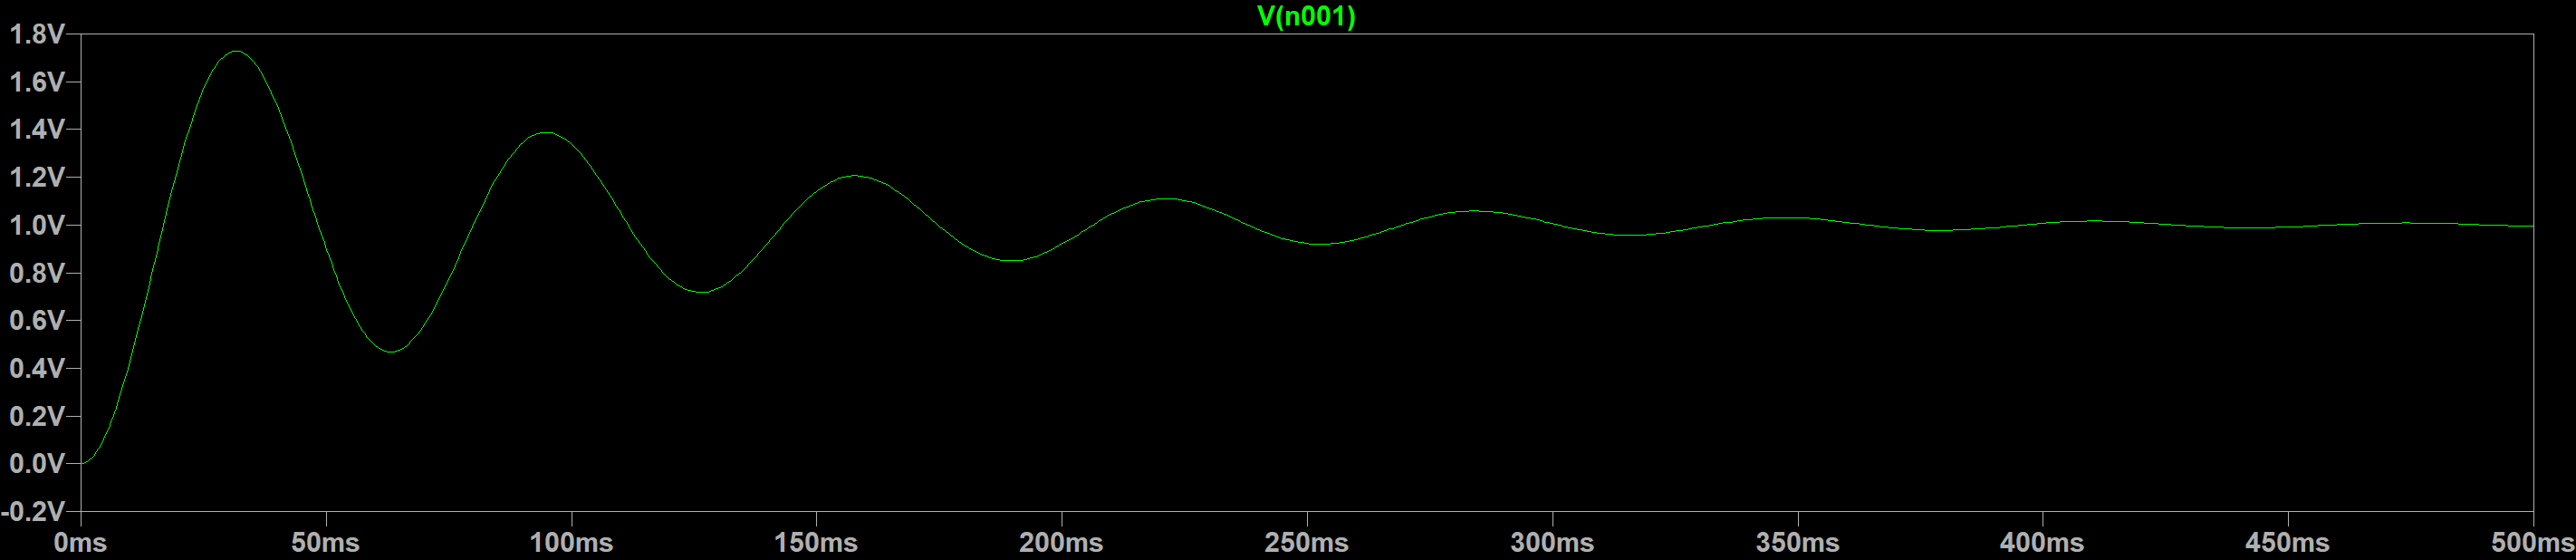
\includegraphics[width=1\linewidth]{partd_unrdamped.png}
    \caption{underdampe R3=40k}
    \label{fig:placeholder}
\end{figure}


\begin{figure}[H]
    \centering
    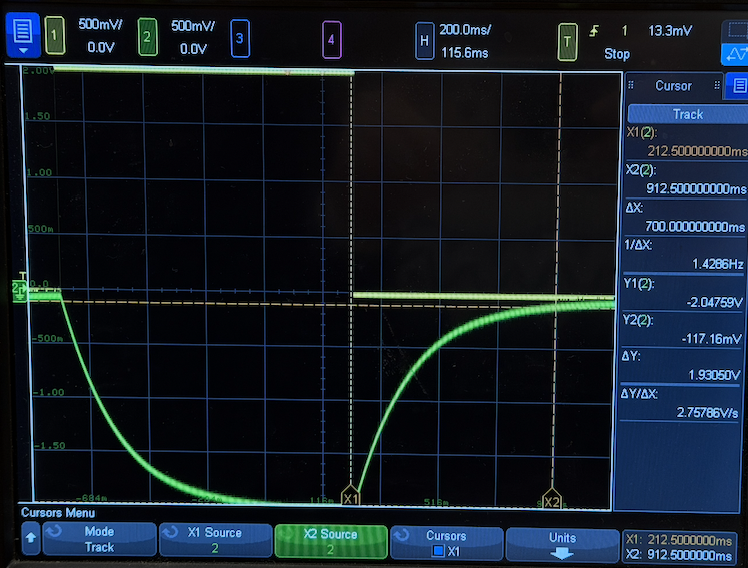
\includegraphics[width=0.5\linewidth]{part1dMsrm_overdamped.png}
    \caption{part 1 d overdamped}
    \label{fig:placeholder}
\end{figure}

\begin{figure}[H]
    \centering
    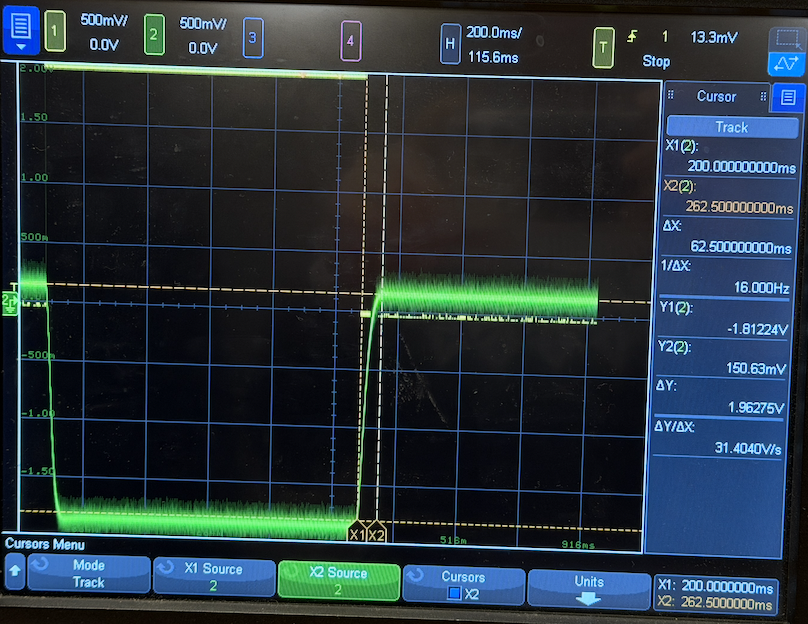
\includegraphics[width=0.5\linewidth]{part1dMsrt_criticallydamped.png}
    \caption{part1 d critically damped}
    \label{fig:placeholder}
\end{figure}



\begin{figure}[H]
    \centering
    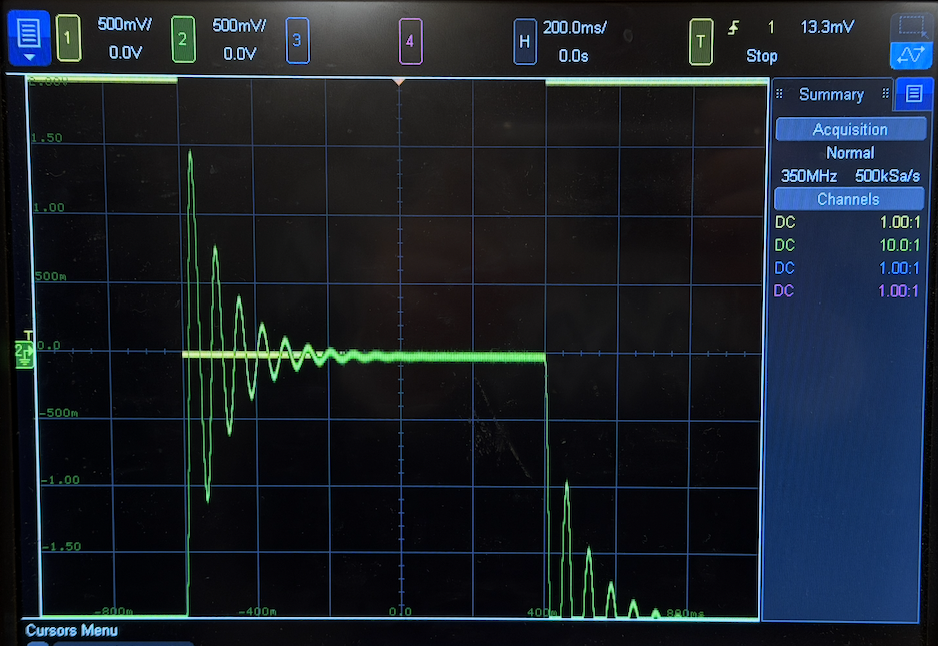
\includegraphics[width=0.5\linewidth]{part1dMsrm_underdamped.png}
    \caption{part 1d underdamped}
    \label{fig:placeholder}
\end{figure}

\begin{figure}[H]
    \centering
    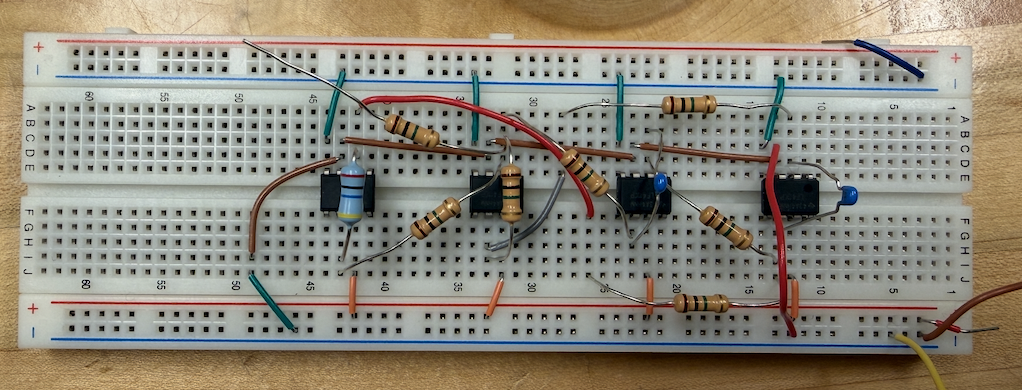
\includegraphics[width=0.5\linewidth]{part1dCircuit.png}
    \caption{1d circuit}
    \label{fig:placeholder}
\end{figure}

\subsection{(e) AC analysis}

\begin{figure}[H]
    \centering
    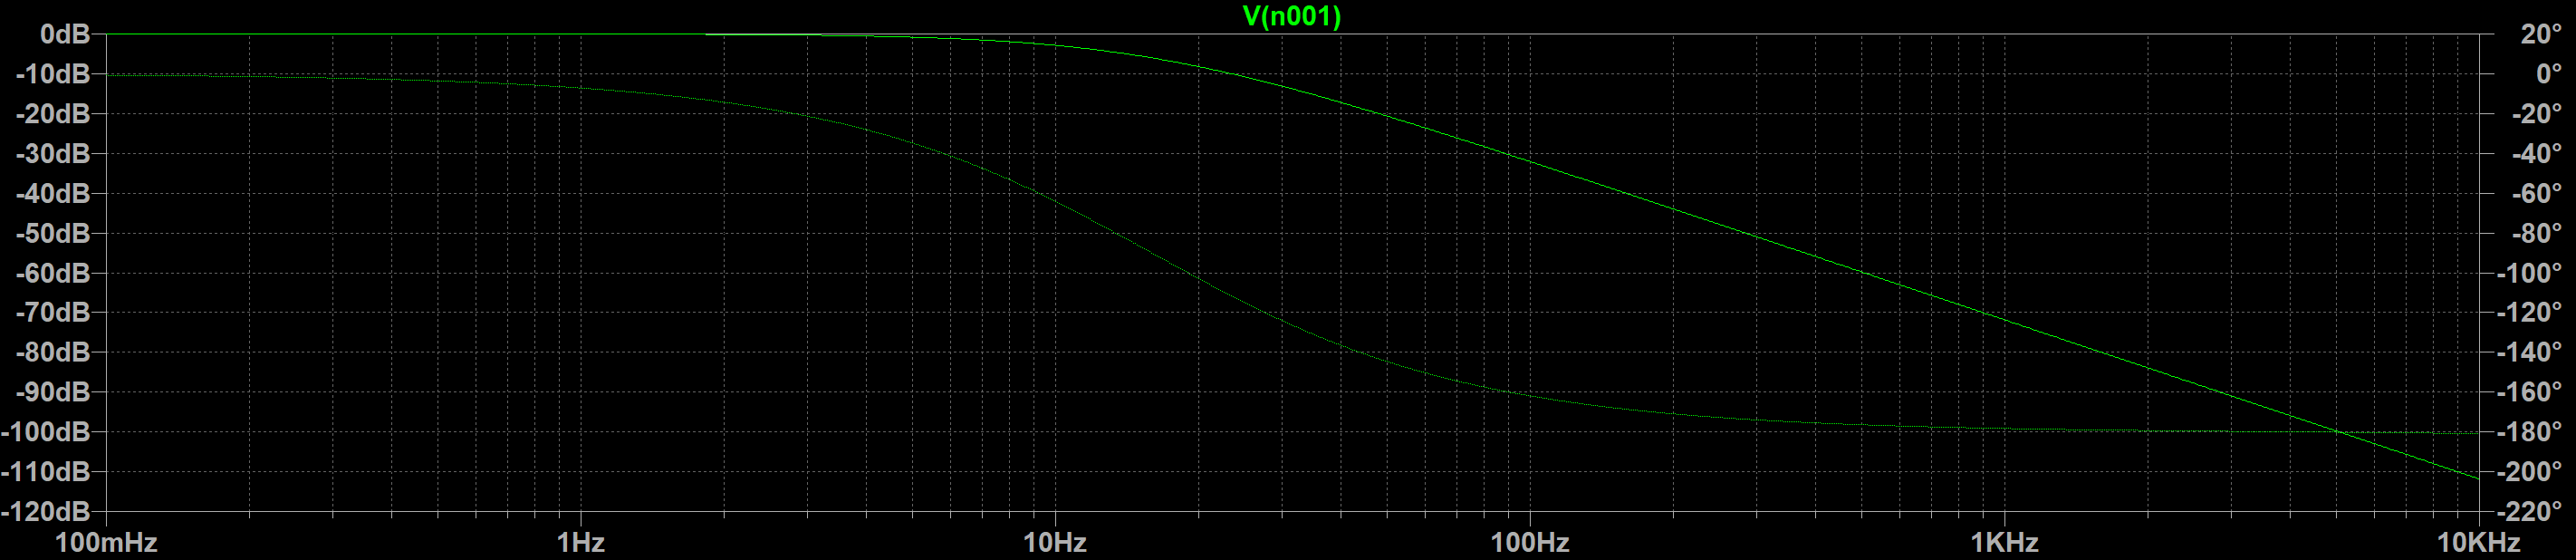
\includegraphics[width=1\linewidth]{part1e.png}
    \caption{Part 1e AC simulation}
    \label{fig:placeholder}
\end{figure}

For critically damped case \((\zeta=1)\), calculated values are :
\begin{itemize}
    \item Low frequencies \(\left(\omega \ll \omega_0\right):|\mathrm{H}(\omega)| \approx 1(0 \mathrm{~dB})\), phase \(\approx 0^{\circ}\)
    \item At \(\omega=\omega_0:\left|\mathrm{H}\left(\omega_0\right)\right|=0.5(-6 \mathrm{~dB})\), phase \(=-90^{\circ}\)
    \item High frequencies \(\left(\omega \gg \omega_0\right):|H(\omega)| \approx\left(\omega_0 / \omega\right)^2\), phase \(\approx-180^{\circ}\)
\end{itemize}


The simulation matches our calculated results.

% \begin{figure}[H]
%     \centering
%     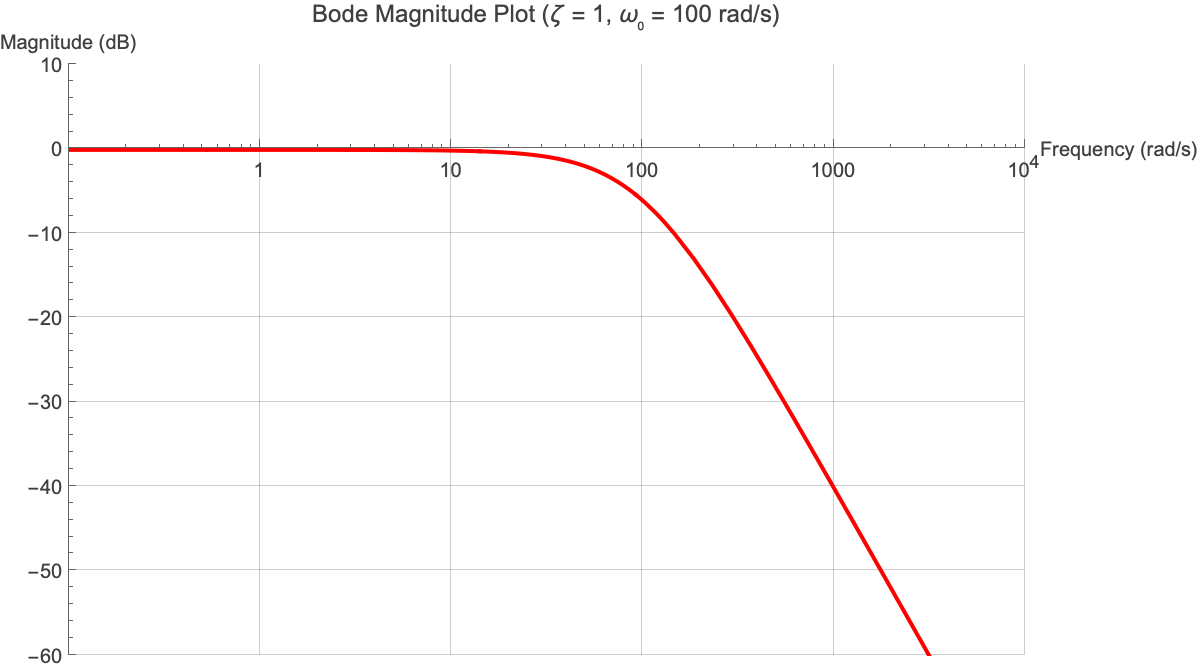
\includegraphics[width=0.5\linewidth]{part1eMathematica_BodeMag.png}
%     \caption{Bode Magnitude Plot}
%     \label{fig:placeholder}
% \end{figure}

% \begin{figure}[H]
%     \centering
%     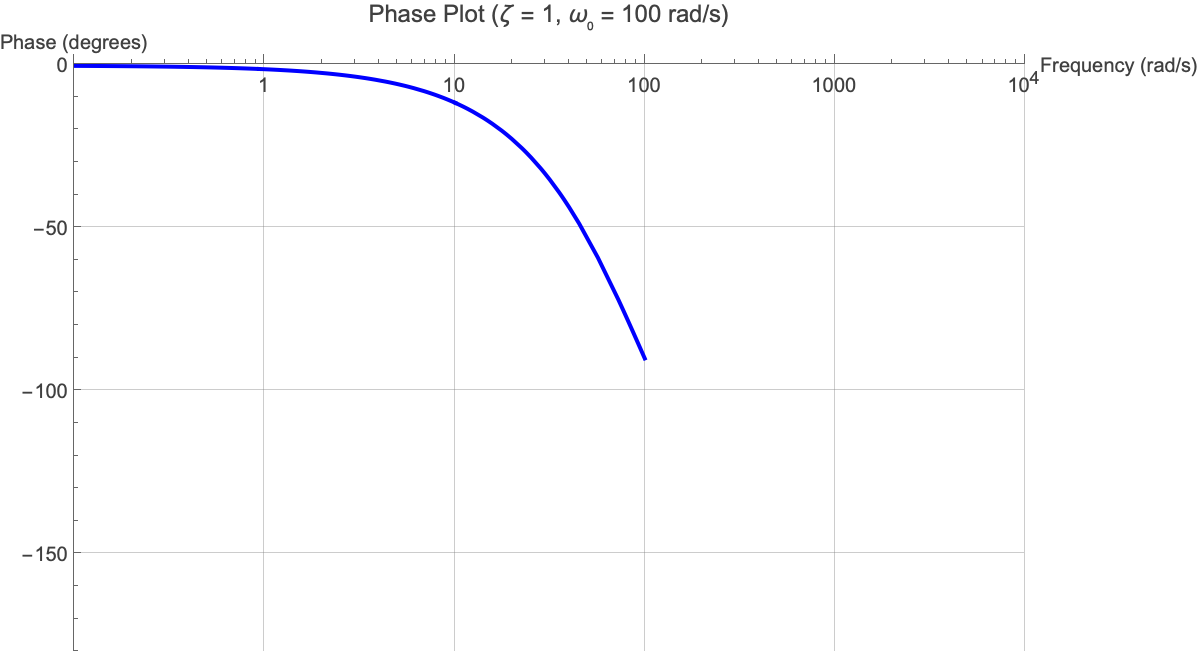
\includegraphics[width=0.5\linewidth]{part1eMathematica_BodePhase.png}
%     \caption{Bode Magnitude Plot}
%     \label{fig:placeholder}
% \end{figure}

\subsection{(f) Q=10}

Starting from part 3, we want to achieve Q=10. So we need to make our \(K_3\) 20 times smaller. Here, I chose \(R_3 = \frac{400k}{20} \Rightarrow K_3/20\)

\begin{figure}[H]
    \centering
    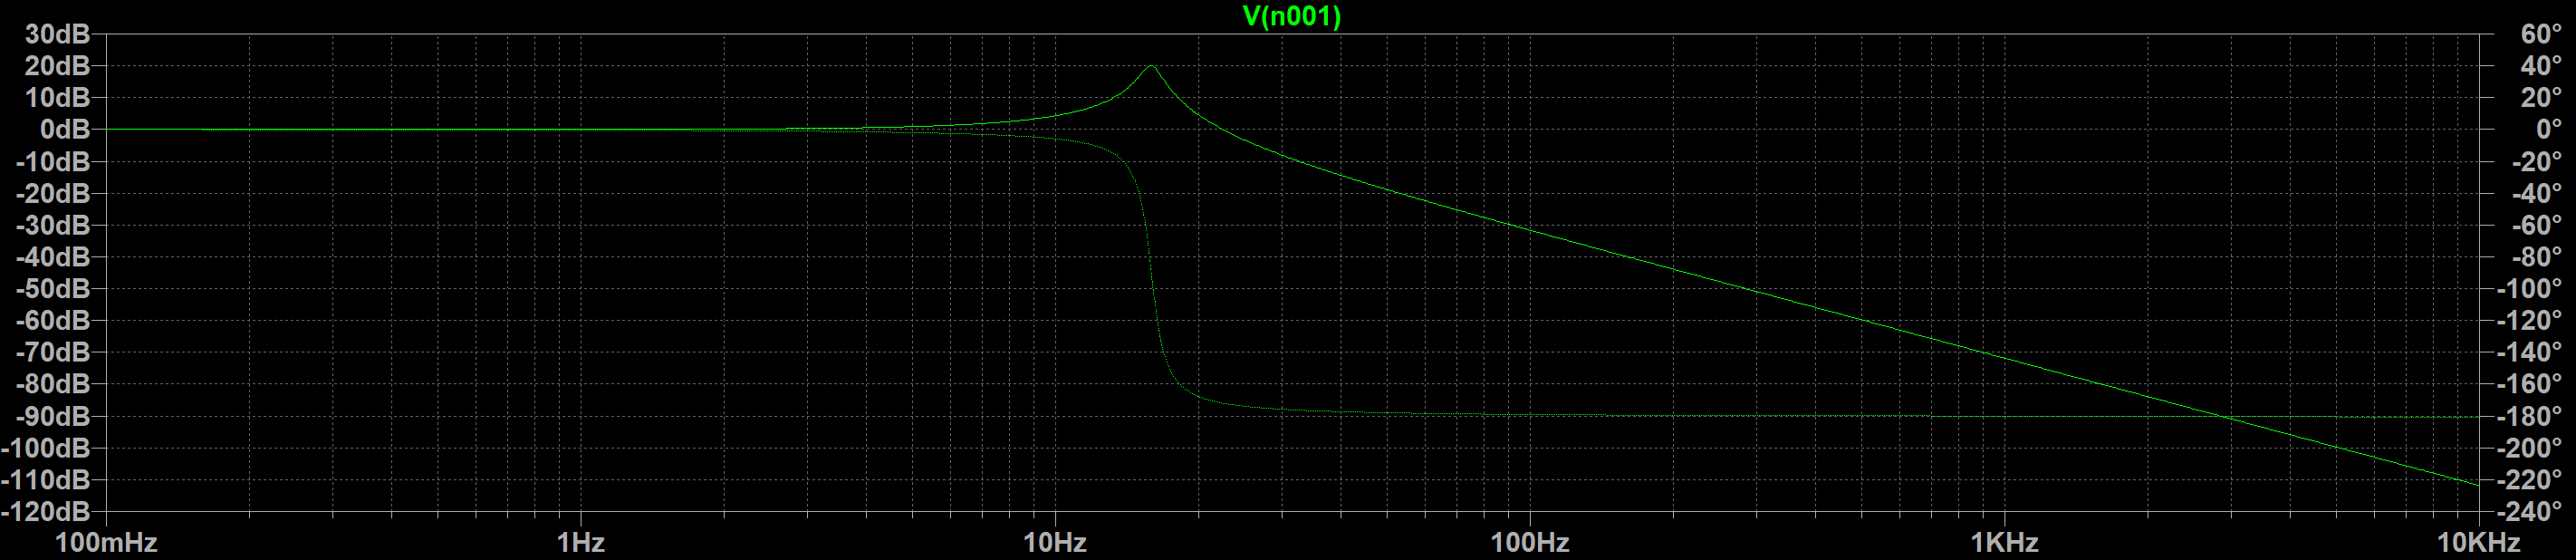
\includegraphics[width=1\linewidth]{part1f_Q10.png}
    \caption{Part 1f Q=10}
    \label{fig:placeholder}
\end{figure}

Sharp resonance peak at \(\approx 99.75 \mathrm{rad} / \mathrm{s}\).
Peak gain \(\approx 10(20 \mathrm{~dB})\) vs \(0.5(-6 \mathrm{~dB})\) for critical.
Much narrower bandwidth (10 rad/s vs broad for critical).
Rapid phase transition near resonance.




\subsection{(g) U1 freq response output}


\begin{figure}[H]
    \centering
    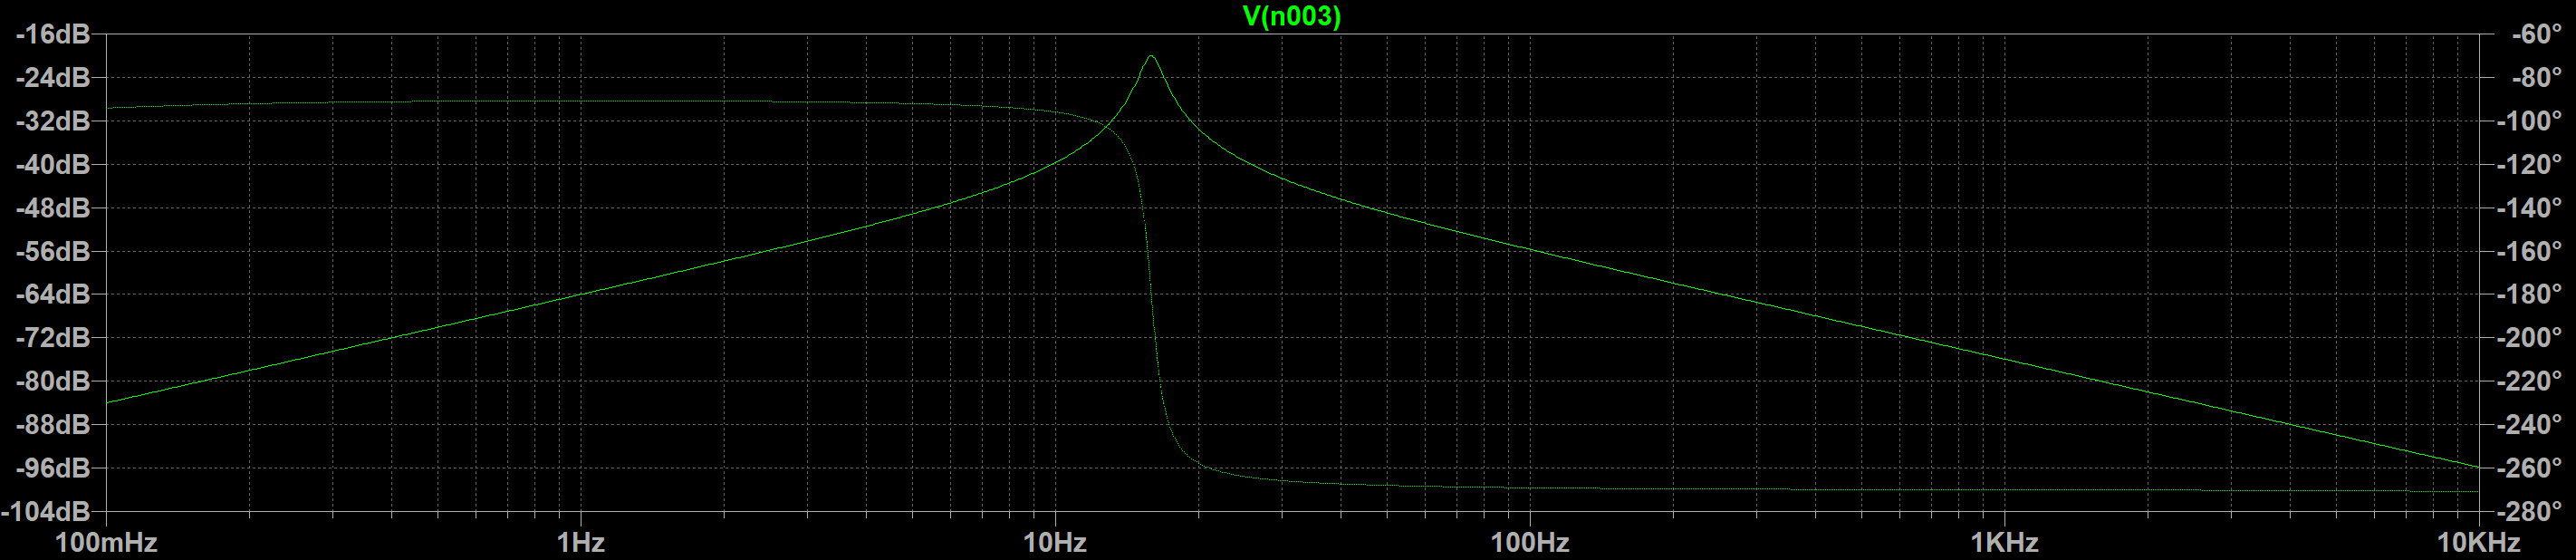
\includegraphics[width=1\linewidth]{part1gU1output.png}
    \caption{U1 output}
    \label{fig:placeholder}
\end{figure}
It's a bandpass filter.

Low frequencies: gain dies out \(\rightarrow 0\) (stopband).
At \(\omega_0=100 \mathrm{rad} / \mathrm{s}\) : peak gain \(=1(0 \mathrm{~dB})\)
High frequencies: gain dies out again → 0 (stopband).
Phase: \(+90^{\circ}\) at low freq \(\rightarrow 0^{\circ}\) at \(\omega_0 \rightarrow-90^{\circ}\) at high freq.
The bandwidth is about \(10 \mathrm{rad} / \mathrm{s}(\)

\subsection{(h) Verifying result}

\[
\begin{aligned}
&\begin{aligned}
& \tau_1=\tau_2=0.01 \mathrm{~s} \\
& K_1=K_2=1 \\
& K_3=0.1(\text { for } Q=10 \text { from part } \mathrm{f}) \\
& \omega_0=100 \mathrm{rad} / \mathrm{s} \\
& Q=10
\end{aligned}\\
&\begin{aligned}
H_{\mathrm{U} 1}(\omega) & =\frac{-j \omega \frac{1}{0.01}}{-\omega^2+j \omega \frac{0.1}{0.01}+\frac{1}{0.01 \times 0.01}} \\
H_{\mathrm{U} 1}(\omega) & =\frac{-j \omega \cdot 100}{-\omega^2+j \omega \cdot 10+10000}
\end{aligned}
\end{aligned}
\]


The U1 output represents the derivative of the state variable (proportional to \(\mathrm{dx} / \mathrm{dt}\) )
and shows the band-pass characteristics with center frequency at \(\omega_0\)
,where peak gain = 1

\subsection{(i) Second response frequency}

\begin{figure}[H]
    \centering
    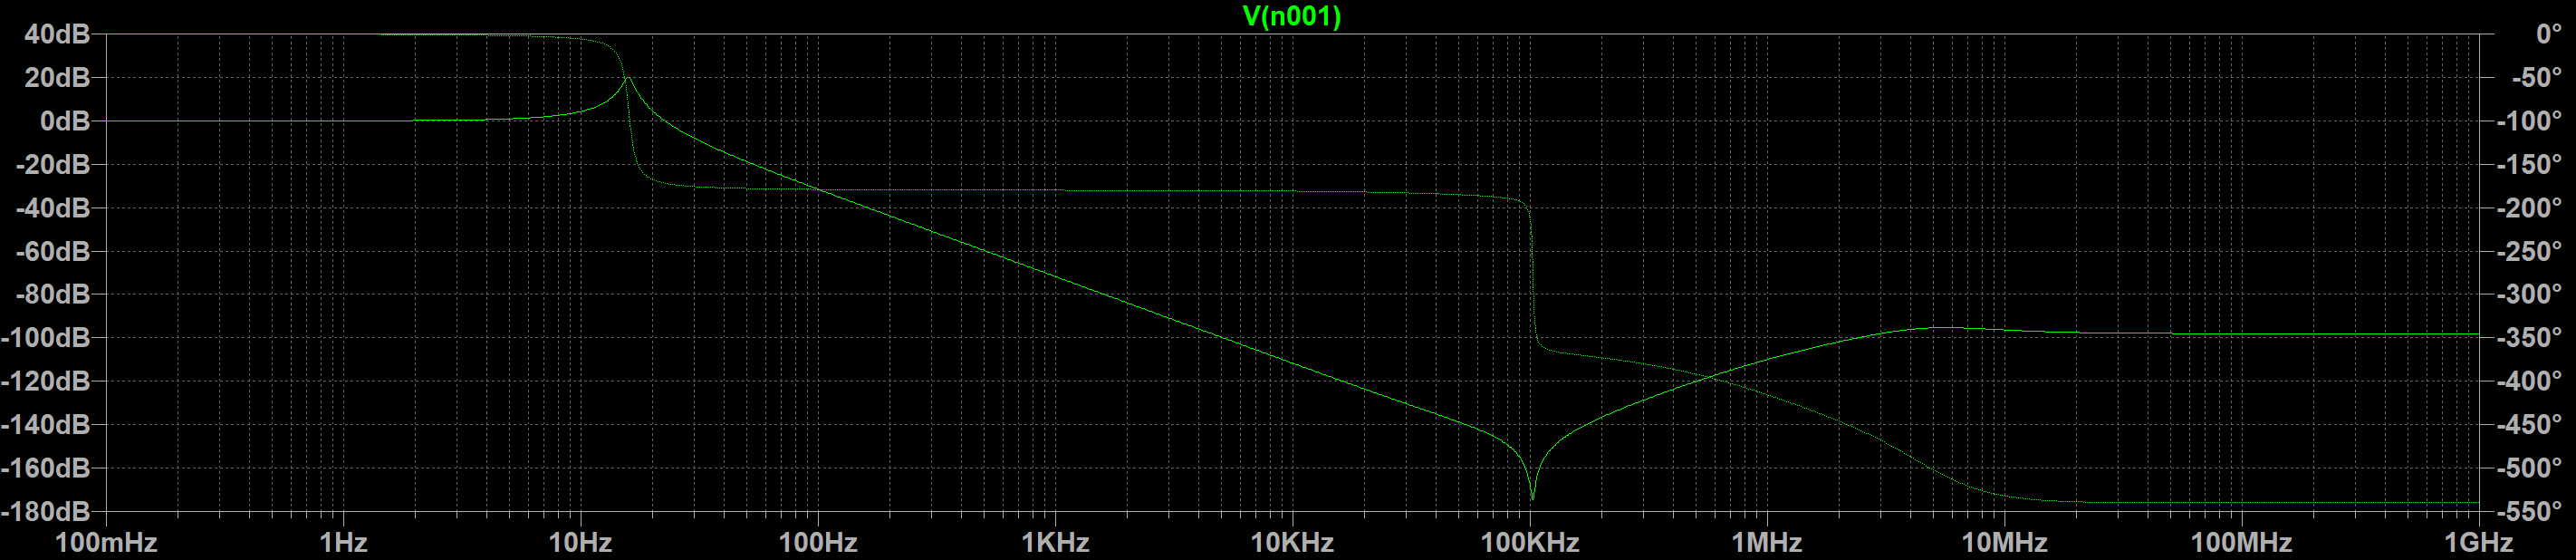
\includegraphics[width=1\linewidth]{part1i1GHz.png}
    \caption{Extend the freq sweep range to find the second resonant freq, which is 100kH}
    \label{fig:placeholder}
\end{figure}


\end{document}